\documentclass[a4paper]{article}

\usepackage[T2A]{fontenc}
\usepackage[russian]{babel}
\usepackage{graphicx}
\usepackage{float}
\usepackage{hyperref}
\usepackage{amsmath, amssymb, diffcoeff, mathtools}
\usepackage{caption}
\usepackage{geometry}
\usepackage{pdfpages}
\usepackage{wrapfig}

\begin{document}

\begin{center}
\textsc{Санкт-Петербургский национальный исследовательский институт информационных технологий, механики и оптики\\[3mm]
Физический факультет} \\[3mm]

\end{center}
\vspace{5mm}
\line(1,0){\textwidth}
\begin{center}
\textbf{ЛАБОРАТОРНАЯ РАБОТА №2.10\\}
\textbf{"Измерение теплоты парообразования воды"}
\end{center}
\vspace{2mm}
\line(1,0){\textwidth}
\vspace{5mm}
\begin{minipage}{0.4\textwidth}
    Группа: Z3144 \\
    Студент: Турчанин Евгений\\
    \vspace{1mm}
\end{minipage}
\hfill
\vspace{1mm}
\line(1,0){\textwidth}


\section{Цели работы}
\begin{enumerate}
    \item Измерение теплоты парообразования воды.
\end{enumerate}


\section{Рабочие формулы и исходные данные}
\begin{itemize}
    \item \textbf{Рабочие формулы}
\end{itemize}
\begin{enumerate}
    \item Количество теплоты, необходимое для превращения жидкости в пар:
        \[ Q = Lm \]
    где $L$ - удельная теплота парообразования, $m$ - масса испарившейся воды.

    \item Мощность, которая уходит в окружающую среду
        \[ N_{\text{окр}} = \frac{cM\Delta t}{\tau} \]
    где $c$ - удельная теплоемкость воды, $M$ - масса воды в сосуде, $\Delta t$ - изменение температуры измерительного модуля, $\tau$ - время, за которое измерительный модуль охлаждается на $\Delta t$.

\pagebreak


    \item Полная мощность:
        \[ N_{\text{полн}} = \frac{U^2}{R} \]
    где U - напряжение, R - сопротивление измерительного модуля.

    \item Полезная мощность:
        \[ P = N_{\text{полн}} - N_{\text{окр}} \]

    \item Работа измерительного модуля
        \[ A = Pt \]
\end{enumerate}

\begin{itemize}
    \item \textbf{Исходные данные}
\end{itemize}
\begin{enumerate}
    \item Измерительный модуль охлаждается на $\Delta t = 10^{\circ}$C за $\tau = 2$ минуты
    \item Воды в сосуде с ТЭНом 1 литр
    \item При 100$^{\circ}$C: R = 82 ОМ, U = 232 В
\end{enumerate}

\section{Экспериментальная установка}

\begin{figure}[H]
    \centering
    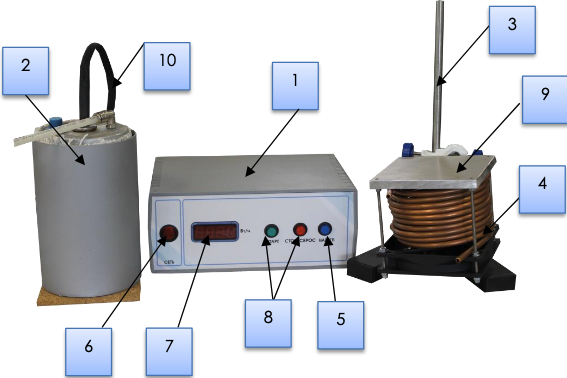
\includegraphics[width=0.9\textwidth]{fig_1.png} 
    \caption{Внешний вид установки.}
    \label{fig:setup}
\end{figure}

\begin{enumerate}
    \item измерительный модуль (счетчик электроэнергии);
    \item сосуд с ТЭНом;
    \item стойка с основанием;
    \item охлаждающий элемент;
\end{enumerate}
\section{Обработка данных}
Для рассчета теплоты парообразования воды используем формулу:
\[
    L = \frac{Q}{m}
\]
где $Q$ рассчитывается по формуле:



\end{document}
